% Created 2021-02-01 Mon 16:02
% Intended LaTeX compiler: pdflatex
\documentclass{SPFIT}
\usepackage[utf8x]{inputenc}
\usepackage[T1]{fontenc}
\usepackage{graphicx}
\usepackage{grffile}
\usepackage{longtable}
\usepackage{wrapfig}
\usepackage{rotating}
\usepackage[normalem]{ulem}
\usepackage{amsmath}
\usepackage{textcomp}
\usepackage{amssymb}
\usepackage{capt-of}
\usepackage{hyperref}
\usepackage{minted}
\usepackage{tikz}
\usepackage{tikz-cd}
\usepackage{bussproofs}
\affiliation{\href{mailto:xzaryb00@stud.fit.vut.cz}{xzaryb00@stud.fit.vut.cz}, \textit{Faculty of Information Technology, Brno University of Technology}}
\date{2020/2021}
\title{Just-in-Time Compilation of the Dependently-Typed Lambda Calculus}
\hypersetup{
 pdfauthor={},
 pdftitle={Just-in-Time Compilation of the Dependently-Typed Lambda Calculus},
 pdfkeywords={},
 pdfsubject={},
 pdfcreator={Emacs 28.0.50 (Org mode 9.3)}, 
 pdflang={English}}
\begin{document}

\PPFinalCopy
\def\myauthor{Jakub Zárybnický}
\def\myabstract{%
When building a programming language, the choice is often between writing a compiler
or an interpreter, a compromise between speed and ease of implementation respectively.
Just-in-time compilation offers a compromise, interpretation combined with
gradual optimization during program runtime.
%
The goal of my goal is to investigate whether just-in-time compilation offers the
same advantages in the dependently-typed lambda calculus just as it does in imperative languages.
%
The implementation environment is the Java Virtual Machine, and in particular
the GraalVM runtime and the Truffle language implementation framework.

In the scope of this term project, I have investigated the relevant
topics of JIT compilation, dependent types, and lambda calculi. I have also
created a reference implementation of the dependently-typed lambda calculus
LambdaPi based on prior work, and started two other implementations---one
a LLVM-based compiler, and a Truffle-based JIT interpreter/compiler.

These three implementations---together with a set of benchmarks---will form
the basis of my thesis and after omtimizations, will either prove or disprove
the usefulness of JIT compilation for the dependently-typed lambda calculus.
}
\startdocument

\section{Introduction}
\label{sec:orgb69e573}
When creating small experimental or research languages, writing a compiler may
be too much effort for the expected gain. On the other hand an interpreter is
usually not as performant as its creators may require for more computationally
intensive tasks.

There is a potential third way, proposed by Yoshihiko Futamura in the 1970s,
called the Futamura projection (or partial program evaluation), wherein an
interpreter is specialized in conjunction with the source code of a program,
yielding an executable. Some parts of the interpreter may be specialized, some
optimized, some left off entirely. Depending on the quality of the specializer,
the gains may be several orders of magnitude.

The goal of my thesis is to evaluate whether the GraalVM/Truffle platform is
suitable enough to act as a specializer for functional languages, in particular
for the dependently-typed lambda calculus.  To illustrate in Figure
\ref{fig:futamora}, the question is whether the path \textit\{Native
Image\textrightarrow Result\} is fast enough compared to the path
\textit{Executable\textrightarrow Result}.

\begin{figure}
\begin{tikzcd}
{} & Program
 \arrow[ld, "Compiler" description, bend right]
 \arrow[dd, "Interpreter" description, bend right=67]
 \arrow[rd, "Partial\ Evaluation" description, bend left]
 \arrow[dd, "JIT" description, bend left=67] & {} \\
Executable \arrow[rd, "Run" description, bend right] & {} & Native\ Image \arrow[ld, "Run", bend left]
 \\ {} & Result & {}
\end{tikzcd}
\caption{Methods of program execution}
\label{fig:futamora}
\end{figure}

Truffle has already been used rather successfully for the (mostly) imperative
languages Ruby, Python, R, Java, and WebAssembly, but (purely-)functional
languages differ in their evaluation model and in particular the required
allocation throughput, so it is still an open question whether GraalVM is a good
enough fit.

The desired outcome---at least, of the first part of my thesis---is a set of
implementations, and a set of benchmarks demonstrating a positive or a negative
result.  If the result is positive, there are many potential follow-up tasks:
implementing a different, more complex language, maybe a language to be
interpreted into the dependently-typed lambda calculus to attempt the approach
implemented in the \emph{Collapsing Tower of Interpreters} \cite{amin2017collapsing},
or experimenting with different runtime models - all depending on the results of
this preliminary proof of concept.

In the best case, the JIT-compiled program would be as close in performance to a
program processed by a hand-crafted compiler as possible (not including JIT
warm-up), and I would spend the second half of my thesis on different topics
(like provably-correct program transformations) instead of hand-optimizing the
primitive operations - I should find out which it is going to be as soon in the
second term as possible.

As far as I am aware, there are no other native just-in-time compiled
implementations of the dependently-typed lambda calculus, with the exception of
the preliminary investigations done by the originator of this idea
\cite{kmett_2019}, although there are a few projects implementing a lambda
calculus directly to the Java Virtual Machine byte code..

\section{Assignment}
\label{sec:org577ba43}
The assignment for the first term was given as follows:
\begin{enumerate}
\item Investigate dependent types, simply-typed and dependently-typed lambda
calculus, and their evaluation models (push/enter, eval/apply).
\item Get familiar with the Graal virtual machine and the Truffle language
implementation framework.
\item Create a parser, and an interpreter for a selected language based on
dependently-typed lambda calculus.
\end{enumerate}

\subsection{Lambda calculus}
\label{sec:org808842e}
The untyped lambda calculus is introduced in the intermediate programming
languages class but I haven't yet encountered its simply- or dependently-typed
variants during my studies.

The untyped lambda calculus is a simple language consisting of just three kinds
of forms: variables, function application, and abstraction.

\begin{figure}[!htpb]
\[\begin{array}{ccll}
e & ::= & x            & \text{variable} \\
  & |   & e_1~e_2      & \text{application} \\
  & |   & \lambda x. e & \text{abstraction}
\end{array}\]
\caption{Untyped lambda calculus}
\end{figure}

The simply-typed lambda calculus adds a fourth kind of a term, type annotation,
and its type language:

\begin{figure}[!htpb]
\[\begin{array}{ccll}
e & ::= & x           & \text{variable} \\
  & |   & e_1~e_2      & \text{application} \\
  & |   & \lambda x. e & \text{abstraction} \\
  & |   & x:\tau     & \text{annotation}
\end{array}\]
\[\begin{array}{ccll}
\tau & ::= & \alpha           & \text{base type} \\
     & |   & \tau\rightarrow\tau' & \text{composite type}
\end{array}\]
\caption{Simply typed lambda calculus}
\end{figure}

The dependently typed lambda calculus merges these two languages together,
simplifying the grammar.

\begin{figure}[!htpb]
\[\begin{array}{ccll}
e & ::= & x           & \text{variable} \\
  & |   & e_1~e_2      & \text{application} \\
  & |   & \lambda x. e & \text{abstraction} \\
  & |   & x:\tau      & \text{annotation} \\
  & |   & *           & \text{the type of types} \\
  & |   & \forall x:\rho.\rho' & \text{dependent function space}
\end{array}\]
\caption{Dependently typed lambda calculus}
\end{figure}

As I was already familiar with the use of dependent types in general programming
e.g.  in Agda or Idris, I took this opportunity to investigate the theoretical
basis of type systems - type systems in general, as used in general programming
languages, their various limitations---like the need to extend System F (System
FC) as used in Haskell to support fully dependent types
\cite{eisenberg2016dependent}, the lambda cube, the expressive power of
different kinds of type systems, and where they are used.

\subsection{GraalVM, Truffle}
\label{sec:org5fac853}
\textbf{GraalVM} is a just-in-time optimizing compiler for the Java bytecode. \textbf{Truffle} is
a set of libraries that expose the internals of the GraalVM compiler, intended
for easy implementation of other languages. So far JavaScript, Python, Ruby, R,
and WebAssembly have Truffle implementations, and therefore can run on the JVM.

GraalVM is also intended to allow creating \emph{polyglot applications} easily,
applications that have their parts written in different languages. It is
therefore easy to e.g. call R to create visualizations for the results of a
Python program, or to call any Truffle language from Java.

There is also the option to compile a \emph{Native Image} to eliminate most program
start-up costs associated with a just-in-time compiler, pre-compiling the
program partially (ahead-of-time).

From the point of view of a programmer, Truffle makes it possible to write an
interpreter, and then slowly add optimizations like program graph rewriting,
node specializations, inline instruction caching or others. This seems like a
good middle ground between spending large amounts of time on an optimized
compiler, and just specifying the semantics of a program in an interpreter that,
however, will likely not run quickly.

While GraalVM/Truffle is open-source and released under GPL v2, an
enterprise edition that claims large performance improvements is released
commercially.

\begin{figure}[!htpb]
\centering
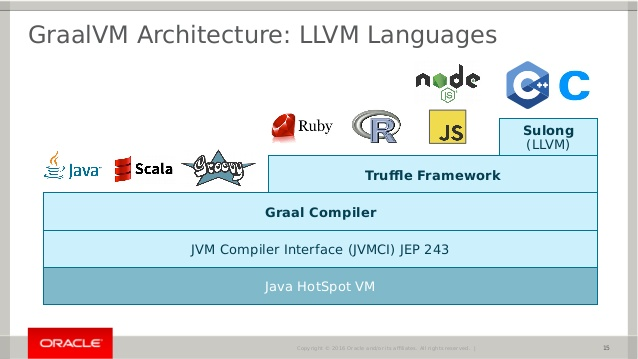
\includegraphics[width=.9\linewidth]{./img/graalvm.jpg}
\caption{GraalVM and Truffle (source: oracle.com)}
\end{figure}

\subsection{LambdaPi implementation}
\label{sec:org9e354c2}
I have implemented a dependently typed lambda calculus called LambdaPi based on
the prior work \emph{A tutorial implementation of a dependently typed lambda calculus}
\cite{loh2010tutorial}. The parser and interpreter are written in Kotlin, where
I will also need to write the JIT implementation. This is a pure interpreter
that will serve as a baseline for future benchmarks.

\begin{listing}[!htpb]
\begin{minted}[]{text}
let const = (\ a b x y -> x)
   :: forall (a :: *) (b :: *) .
      a -> b -> a
\end{minted}
\caption{The constant function in LambdaPi}
\end{listing}

I have also translated parts of the language to Truffle, starting a second
language implementation that will become the baseline JIT implementation, as
well as preparing the groundwork for a third implementation, a compiler based on
the LLVM.

Push/enter and eval/apply, the last items of the first task of my assignment,
are relevant here, they are the two options for expressing partially-applied
function (PAP) objects on the heap. While they are mostly equivalent in
performance when applied to compilers \cite{marlow2004making}, they differ in
how difficult their implementation is, and their performance as part of Truffle
will likely not be equal.  A part of my work next term will be figuring out how
well they map to the execution model of Truffle.

\section{Conclusions}
\label{sec:org3f13b07}
The next step is finalizing the basic Truffle implementation, applying the
specializations as recommended by the Truffle documentation, and investigating
other possible optimizations, especially pertaining to trampolining and
specializing recursive functions.

There are a few different functional languages that compile directly to the JVM
bytecode, and these may serve as inspiration as to how the JVM limits
them---especially given that the JVM does not directly support tail calls.

After this, creating a set of benchmarks written in LambdaPi is the next
step. Any further work will depend on the results of these benchmarks, after
seeing how the performance of the individual implementations differs.

\phantomsection
\bibliographystyle{bib-styles/enplain}
\bibliography{2021-SP-TruffleJIT-bib}
\end{document}